%\documentclass{cmspaper}
%\begin{document} 

\section{Data-driven techniques for background estimate} \label{sec:bkgStudy}
After the event selection the dominant number of SM background events in the two electron 
and two jet sample (eejj sample) comes from $t\bar{t}$ and $Z/\gamma$+jet processes, 
as summarized in table \ref{tab:EventSelSummary}. 
Sections~\ref{sec:ttbarControlSample} and~\ref{sec:ZcontrolSample} 
describe data-driven techniques used to estimate the absolute 
normalization for these two backgrounds, and the shape of selection variable 
distributions for $t\bar{t}$ background using control samples. 
%These shapes are used in a fit to the data to extract the number of signal events, as described 
%in section \ref{sec:signalExtraction}. 
The methods for background estimation described here are based on data and complemented by some Monte Carlo information. 
They are therefore particularly suited for first data taking when confidence that the MC describes
the data well is expected to be limited.

For our analysis, the main properties of a control sample to estimate a background $X$ are:
\begin{itemize}
%
\item to be enriched in $X$ events.
%
\item to be independent from the signal sample;
%
\item to have similar topology of the $X$ events in the signal sample (i.e. eejj sample) 
concerning a given set of reconstructed selection variables under investigation;  
%concerning a given set of reconstructed quantities under investigation;  
%
\end{itemize}
%
The control samples for the $t\bar{t}$ and $Z/\gamma$+jet backgrounds discussed below both satisfy 
these three conditions.
Different considerations are applied to estimate the QCD multi-jet background as described in 
Section~\ref{sec:QCDBackground}.

% NOTE: the more detailed discussion on different amount of background should be discussed in the section Event Selection 
% when you show the table with the number of selected events

%The four main source of background events that pass the High Level Trigger are ttbar, Z+jets, QCD and W+jets.  The application of the electron isolation criteria sufficiently limits the number of fake electrons in the offline selection that the QCD and W+jets background are negligible.  The small contribution of the events with fake electrons from the QCD and W+jet channels can be seen in figure~\ref{fig:Mej_allComb}.

\subsection{$t\bar{t}$ background control sample} \label{sec:ttbarControlSample}

The normalization and the shape of the main selection variable distributions for 
$t\bar{t}$ events can be estimated directly from data using a control sample. 
The basic idea is to select events that are independent from the eejj sample, and have, for the main selection variables, 
shape and resolution similar to the $t\bar{t}$ component in the eejj sample.

Very strong constraints from rare processes exist on leptoquarks with
couplings to both electrons and muons.
Therefore a good control sample can be obtained by using the same selection criteria applied for the eejj sample, but 
requiring at least one electron and one muon (e$\mu$jj sample) instead of at least 2 electrons 
in the final state in addition to the two jets. 
For $t\bar{t}$ events, the selection variable distributions of the e$\mu$jj and the eejj samples
are expected to be very similar in shape since the kinematics of the process does not depend 
on the nature of the lepton. Figure~\ref{fig:ttbar} shows a good agreement between 
the shape of $M_{lj}$ and $S_{T}$ distributions with the current MC statistics available. Similar agreement 
is found also for the other reconstructed kinematic variables used in the selection. 

The e$\mu$jj sample is dominated by $t\bar{t}$ events, as shown in Figure~\ref{fig:emujjContamination} 
with a small contamination estimated from MC of less than 5\% (with $S_{T}$ cut of 300 GeV), 
mainly from di-boson events (for $W$+jets and $Z/\gamma$+jets contributions, the statistical 
uncertainties are large, around 100\%, due to limited MC statistics). 
The QCD multi-jet background contamination in the e$\mu$jj sample is expected to be small, as described 
in Section~\ref{sec:QCDBackground}. 
%The QCD multi-jet background contamination in the e$\mu$jj sample is not evaluated here, and it's expected to be small. 
%The MC statistics of QCD multi-jet sample is not sufficient to perform a reasonable estimate at this stage, although 
%it seems to confirm the expectation; the plans of using data driven methods to estimate such background 
%will be discussed later in Section~\ref{sec:QCDBackground}. 
For $t\bar{t}$ events, the e$\mu$jj sample with 100 pb$^{-1}$ of data 
is expected to have about 66, 11, and 5 events, respectively for an $S_{T}$ cut of 300, 520, and 620 GeV.

For a sample of $t\bar{t}$ events at generator level, the number of e$\mu$jj events is expected to be
exactly two times the number of eejj events, considering all the possible combinations of the $W$ decays.
In general, the trigger filter, the offline selection, and the different reconstruction efficiency,
acceptance and $p_{T}$ resolution between electron and muon put a bias in the relative amount of eejj 
and e$\mu$jj events. 
In this analysis the effect of the different reconstruction efficiency between electrons and muons 
(which is the dominant effect for the current selection) 
is considered, in order to estimate the number of eejj in the signal sample directly from 
the size of the e$\mu$jj control sample. The estimate of the number of $t\bar{t}$ events in the eejj sample, 
$N_{eejj}^{est.}$, is extracted from the e$\mu$jj sample according with the relation 

\begin{equation} \label{formula:NeejFromNemujj}
N_{eejj}^{est.} = \frac{1}{2}\sum_{p_{T}^{\mu}} N_{e\mu jj}(p_{T}^{\mu}) \times R(p_{T}^{\mu}) \quad , 
\end{equation}

where $N_{e\mu jj}(p_{T}^{\mu})$ is the $p_{T}$ distribution for e$\mu$jj events of the muon  
with largest transverse momentum, and $R(p_{T})$ is the ratio between electron 
and muon reconstruction efficiencies as a function of lepton $p_{T}$. The ratio $R(p_{T})$ has been obtained 
using a MC FullSim sample of Z+jets events with an equivalent integrated luminosity of about 275 pb$^{-1}$.
The value of $R(p_{T})$ is found to be between 0.85-0.95 for $30 < p_{T} < 500$ GeV.
Once real data becomes available this ratio could be obtained with $tag\&probe$ method using $Z \rightarrow ee$ and 
$Z \rightarrow \mu\mu$ events (see Section \ref{sec:electronEfficiency}).
A closure test of the method is performed using a MC sample of $t\bar{t}$ events. 
Table~\ref{tab:emujjClosureTest} shows the good agreement within statistical uncertainties between 
the $N_{eejj}^{est.}$, calculated from Equation~\ref{formula:NeejFromNemujj}, 
and the prevision from MC, $N_{eejj}$, for samples selected with a loose $S_{T}$ cut of 300 GeV.   

%{\sl Discussion of how clearly this plot shows similar shape and how this will be used}
%
\begin{figure}[htb]
  \begin{center}
  \begin{tabular}{cc}
  \resizebox{8cm}{!}{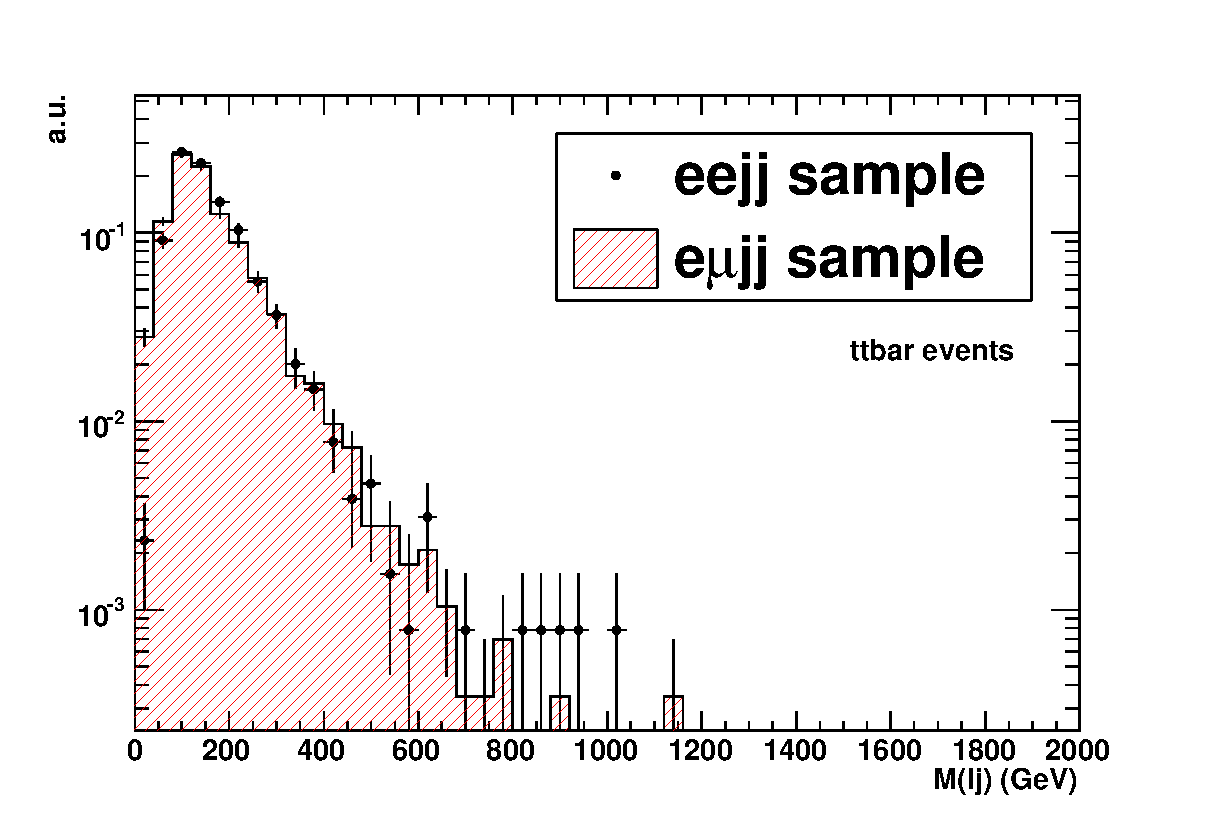
\includegraphics{plots/ttbarStudies/Mlj_eejj_VS_emujj_ttbar_STcut300.eps}} &
  \resizebox{8cm}{!}{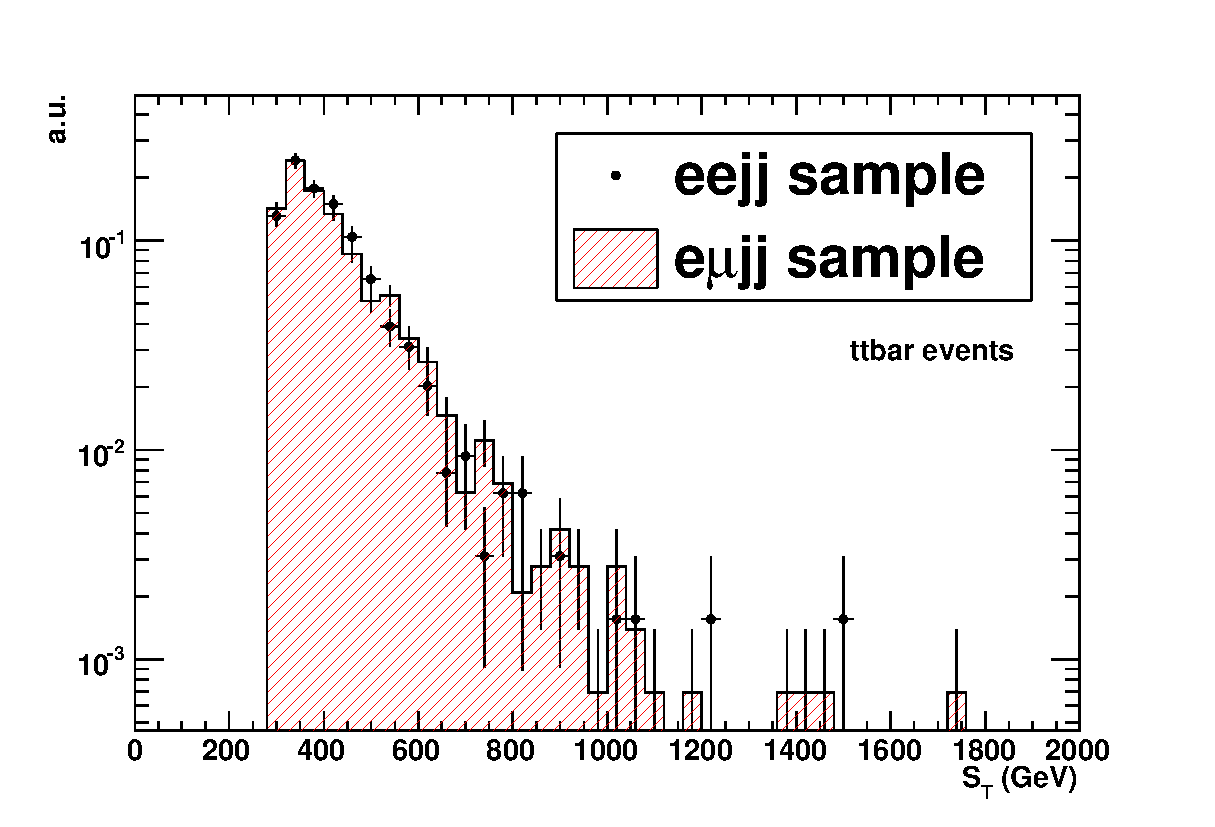
\includegraphics{plots/ttbarStudies/ST_eejj_VS_emujj_ttbar_STcut300.eps}} \\
  \end{tabular}
  \caption{\small \sl Distributions of the lepton-jet invariant mass (left) and $S_{T}$ for the eejj and the e$\mu$ samples, for $t\bar{t}$ events.
  Baseline selection criteria (cut 1,2,3) 
  described in Section~\ref{sec:eventSelection} are applied, but the $S_{T}$ cut has been set to 300 GeV.}
  \label{fig:ttbar}
  \end{center}
\end{figure}
%
\begin{figure}[htb]
  \begin{center}
  \begin{tabular}{cc}
  \resizebox{10cm}{!}{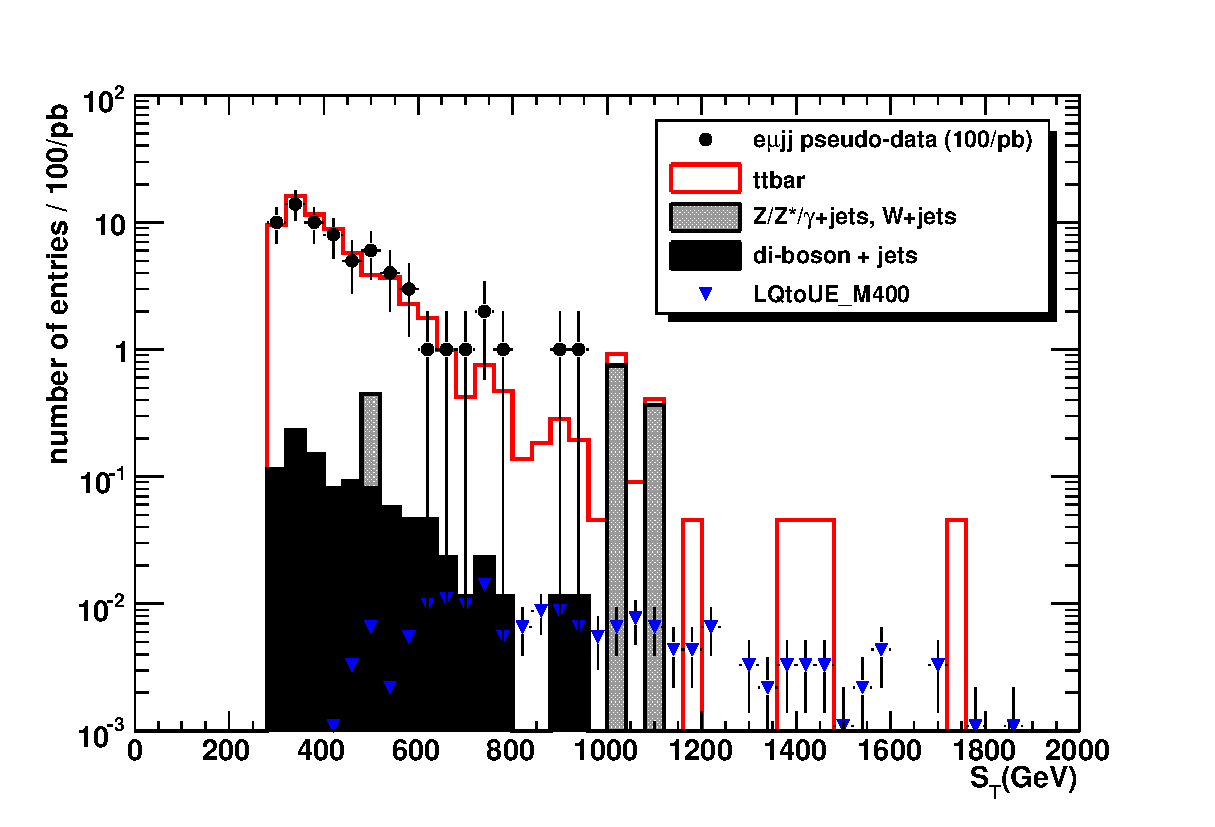
\includegraphics{plots/ttbarStudies/ST_emujj_100pb-1_STcut300.eps}} 
  \end{tabular}
  \caption{\small \sl Distribution of the $S_{T}$ variable for e$\mu$jj sample
    for different background components. 
    Histogram of signal events (at 400~GeV LQ mass) is also added. 
    Baseline selection criteria (cut 1,2,3) described in Section~\ref{sec:eventSelection} 
    are applied, but the $S_{T}$ cut has been set to 300 GeV.
    The background histograms are summed on top of each other.
    Black dots indicate pseudo data randomly generated according to 
    the total background distribution, and assuming 100 pb$^{-1}$ of data.}
  \label{fig:emujjContamination}
  \end{center}
\end{figure}
%
\begin{table}[htbp]
  \begin{center}
    \begin{tabular}{|c|c||c|} \hline
      $N_{eejj}$      & $N_{e\mu jj}$   & $N_{eejj}^{est.}$ \\ 
      \hline
      29.4 $\pm$ 1.2  & 65.9 $\pm$ 1.8  & 29.5 $\pm$ 0.8    \\
      \hline
    \end{tabular}
  \end{center}
  \caption{\small \sl $N_{eejj}$ ($N_{e\mu jj}$) is the 
    MC prediction on the number of 
    $t\bar{t}$ events in the eejj 
    (e$\mu$jj) sample with $S_{T}$ cut of 300 GeV, 
    $N_{eejj}^{est.}$ is the number of eejj $t\bar{t}$ events 
    estimated from the e$\mu$jj sample by using 
    Equation~\ref{formula:NeejFromNemujj}.} 
  \label{tab:emujjClosureTest}
\end{table}
%
%\begin{table}[htbp]
%  \label{tab:emujjClosureTest}
%  \begin{center}
%    \begin{tabular}{|l|c|} \hline
%      $N_{eejj}$ & 29.4 $\pm$ 1.2 \\ \hline
%      $N_{e\mu jj}$ & 65.9 $\pm$ 1.8 \\ \hline \hline
%      $N_{eejj}^{est.}$ &  29.5 $\pm$ 0.8 \\ \hline
%    \end{tabular}
%    \caption{\small \sl $N_{eejj}$ ($N_{e\mu jj}$) is the 
%      MC prediction on the number of 
%      $t\bar{t}$ events in the eejj 
%      (e$\mu$jj) sample with $S_{T}$ cut of 300 GeV, 
%      $N_{eejj}^{est.}$ is the number of eejj $t\bar{t}$ events 
%      estimated from the e$\mu$jj sample by using 
%      Equation~\ref{formula:NeejFromNemujj}. 
%    } 
%  \end{center}
%\end{table}

\clearpage

\subsection{$Z/\gamma$+jet background control sample} \label{sec:ZcontrolSample}

A control sample for $Z/\gamma$+jet background estimation (eejjAtZ sample) 
can be obtained by using the same selection criteria applied for the eejj sample except 
the $M_{ee}$ cut, which is modified to select events with a real $Z$ boson reconstructed 
($80\mbox{ GeV} < M_{ee} < 100\mbox{ GeV}$). This control sample is an almost pure sample of  
$Z/\gamma$+jet events as shown in Figure~\ref{fig:eejjAtZContamination}   
( less than 4\% contamination dominated by $t\bar{t}$ events, for $S_{T}$ cut of 300 GeV), 
since the cross section of the process is resonant at the Z mass.
The signal contamination is less than 10\% for all $S_{T}$ cuts considered.  
%the eejjAtZ sample is independent from the eejj signal sample by construction. 
For $Z/\gamma$+jet events, the eejjAtZ sample with 100 pb$^{-1}$ of data 
is expected to have about 129, 21, and 11 events, respectively for an $S_{T}$ cut of 300, 520, and 620 GeV.

The rescaling of the control sample can be obtained with an hybrid method which combines the eejjAtZ data with 
MC information. Once real data is available the eejjAtZ sample can be selected. 
The number of $Z/\gamma$+jet events in the eejj signal sample ($M_{ee}>100$ GeV) can be estimated by

\begin{equation} \label{formula:NeejjZ}
N_{eejj}^{Z} = N_{eejjAtZ} \times R_{OffZ/AtZ} \quad , 
\end{equation}

where $N_{eejjAtZ}$ is the number of events in the eejjAtZ control sample, and 
$R_{OffZ/AtZ}$ is the ratio between the number of $Z/\gamma$+jet events 
with $M_{ee} > 100\mbox{ GeV}$ (OffZ events) and $80\mbox{ GeV} < M_{ee} < 100\mbox{ GeV}$ 
(AtZ events) that have passed all the other selection criteria.
In this analysis the value of $R_{OffZ/AtZ}$ is determined directly from MC.
The motivations that justify this approach are discussed below:
%
\begin{itemize}
%
\item those theoretical uncertainties that are independent 
on the value of two electron invariant mass cancel in the ratio.
Generator level studies will be performed 
in future upgrades of the analysis to quantify the
remaining uncertainties on the value of $R_{OffZ/AtZ}$, 
by using different sets of PDFs and various MC generators;
%
%and eejjAtZ data is used to rescale the $Z/\gamma$ MC sample, 
%thus setting the correct background normalization;
%
\item for inclusive $Z/\gamma \rightarrow ee$ production (with no jets), 
the MC is expected to predict the value of the ratio $R_{OffZ/AtZ}$ with small 
uncertainty (dominated by PDF uncertainties). 
The data-MC comparison will be done with real data by calculating 
the ratio $R_{OffZ/AtZ}$ using a control sample with only two electrons 
(which is expected to be dominated by Drell-Yan events 
up to values of $M_{ee}$ of about one TeV~\cite{HEEPNOTE});
%
\item the next step will be to compare the distributions of reconstructed selection 
variables between eejjAtZ data and MC to check the agreement in the control region.
It's expected to have more confidence in the MC extrapolation 
from the control region to the signal region ({\it id est} the estimation of the ratio $R_{OffZ/AtZ}$), 
if the event kinematics in the two regions is not dramatically different, in particular for the 
hadronic part of the process.
Figure~\ref{fig:BjjSTJetseejjAtZvsOffZ}
show the distributions of the scalar sum of $p_{T}$ of the two leading jets ($S_{T}^{jets}$) 
and the distribution of the velocity of the jet-jet system ($\beta_{jj} = v_{jj}/c$) 
for $Z/\gamma$+jet events, 
%show the distributions of the scalar sum of $p_{T}$ of the two leading electron ($S_{T}^{ele}$) 
%and the two leading jets ($S_{T}^{jets}$) for $Z/\gamma$+jet events, 
in both the signal region (eejjOffZ sample) and the control region (eejjAtZ control sample). 
%A significant discrepancy is observed 
%in the $S_{T}^{ele}$ distribution; this should not represent 
%a problem for the MC extrapolation, since the Electro-Weak part of the process 
%is well predicted, and the expected agreement could be directly checked with a control sample 
%of two electrons (as described in the previous bullet).
It's comforting that the two distributions are in agreement, 
which is an indication that the hadronic part of the $Z/\gamma$+jet process 
(the one with largest theoretical uncertainties) is similar between 
the signal and the control region.  
%
\end{itemize}

The method described by Equation~\ref{formula:NeejjZ} is applied assuming 100 pb$^{-1}$ 
of data. In this MC exercise, the number of events expected in the eejjAtZ control sample, $N_{eejj}^{Z}$, 
is obtained from the FullSim MC sample of $Z/\gamma$+jet (although this will come directly from data).
The statistical uncertainty on this number is assumed $\sqrt{N_{eejj}^{Z}}$, which is 
the counting error on the data.
The ratio $R_{OffZ/AtZ}$ is extracted from the FastSim MC sample of $Z/\gamma$+jet events.
Figure~\ref{fig:ZJetRatioAndMeeFastVSFull} shows the agreement of the 
$M_{ee}$ distribution between FastSim and FullSim, and the value of the inverse of $R_{OffZ/AtZ}$ 
as a function of different $S_{T}$ cuts, obtained from FastSim. 
The results of the application of the method are shown in Table~\ref{tab:ZjetClosureTest}.
The number of $Z/\gamma$+jet in the eejj sample estimated using the data driven method 
($N_{eejj}^{Z}$ from Equation~\ref{formula:NeejjZ}) 
is in agreement with the number of $Z/\gamma$+jet events in the eejj sample directly 
obtained by applying the eejj selection on the FullSim MC sample ($N_{eejjOffZ}$).

%Figure~\ref{fig:zjet} shows the good agreement between eejjAtZ and eejj samples for both the shapes of $M_{ej}$ 
%and $S_{T}$ distributions, using a large FastSim MC sample of $Z/\gamma$+jet events. 
%The agreement observed can be interpreted as the consequence of the 
%weak correlation between the two reconstructed quantities $M_{ej}$ ($S_{T}$) and $M_{ee}$ for selected events, as shown in 
%Figure~\ref{MejVsMeeCorrelation} (Figure~\ref{STVsMeeCorrelation}).

\begin{figure}[htb]
  \begin{center}
  \begin{tabular}{cc}
  \resizebox{10cm}{!}{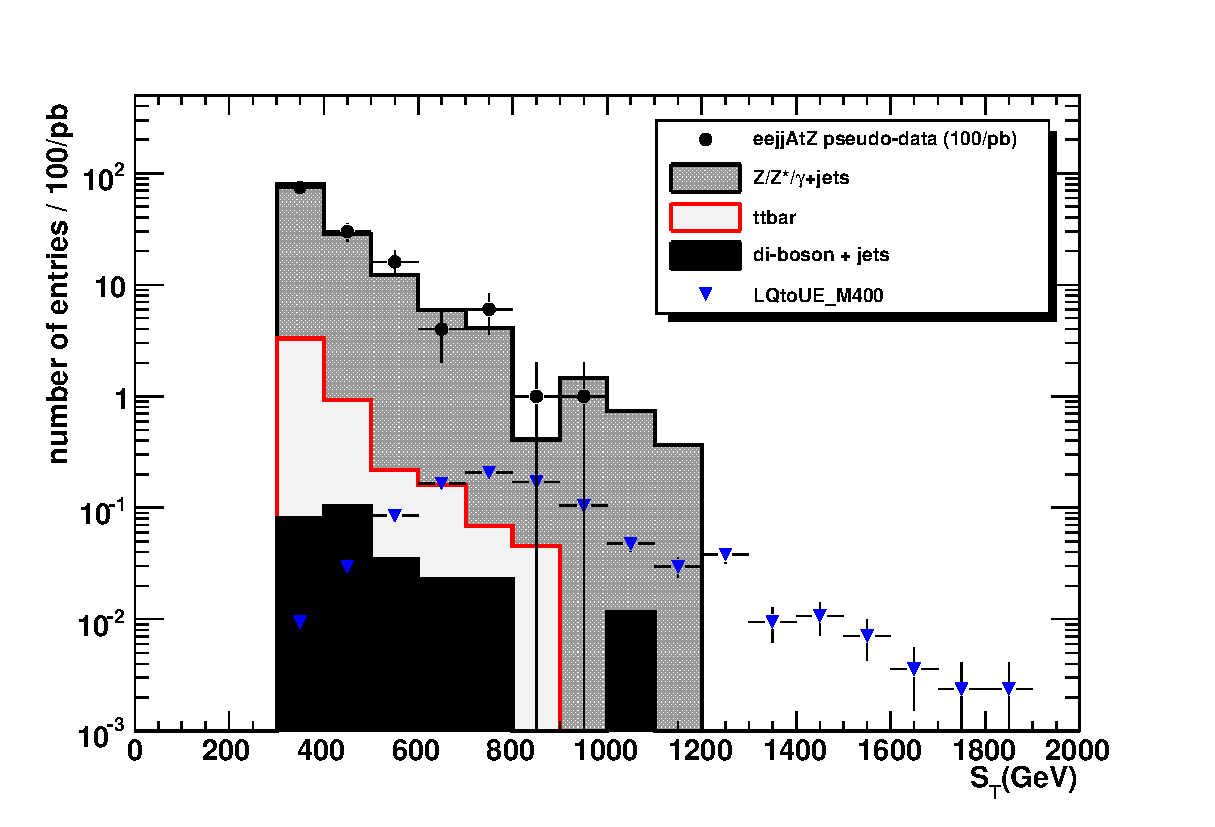
\includegraphics{plots/ZjetStudies/ST_100InVpb_eejjAtZ_looseSTcut_MeeInverted_WithLQ400.eps}} \\ 
  \end{tabular}
%  \caption{\small \sl Distribution of the $p_{T}$ at generator level of the electron pair ($p_{T}$ of the boson) 
%    for $Z/\gamma$+jet events in the signal eejj sample 
%    (cut 1,2,3,4)
%    and the control sample (cut 1,2,4 + $80\mbox{ GeV} < M_{ee} < 100\mbox{ GeV}$), for $Z/\gamma$+jet events.}
  \caption{\small \sl Distribution of the $S_{T}$ variable for eejjAtZ sample
    for different background components. 
    Histogram of signal events (at 400~GeV LQ mass) is also added. 
    Baseline selection criteria (cut 1,2) described in Section~\ref{sec:eventSelection} 
    are applied, $S_{T}$ cut has been set to 300 GeV, 
    cut on $M_{ee}$ is modified to select real Z bosons ($80\mbox{ GeV} < M_{ee} < 100\mbox{ GeV}$).
    The background histograms are summed on top of each other.
    Black dots indicate pseudo data randomly generated according to 
    the total background distribution, and assuming 100 pb$^{-1}$ of data.}
  \label{fig:eejjAtZContamination}
  \end{center}
\end{figure}
%
%
%
\begin{figure}[htb]
  \begin{center}
  \begin{tabular}{cc}
    a.
    \resizebox{8cm}{!}{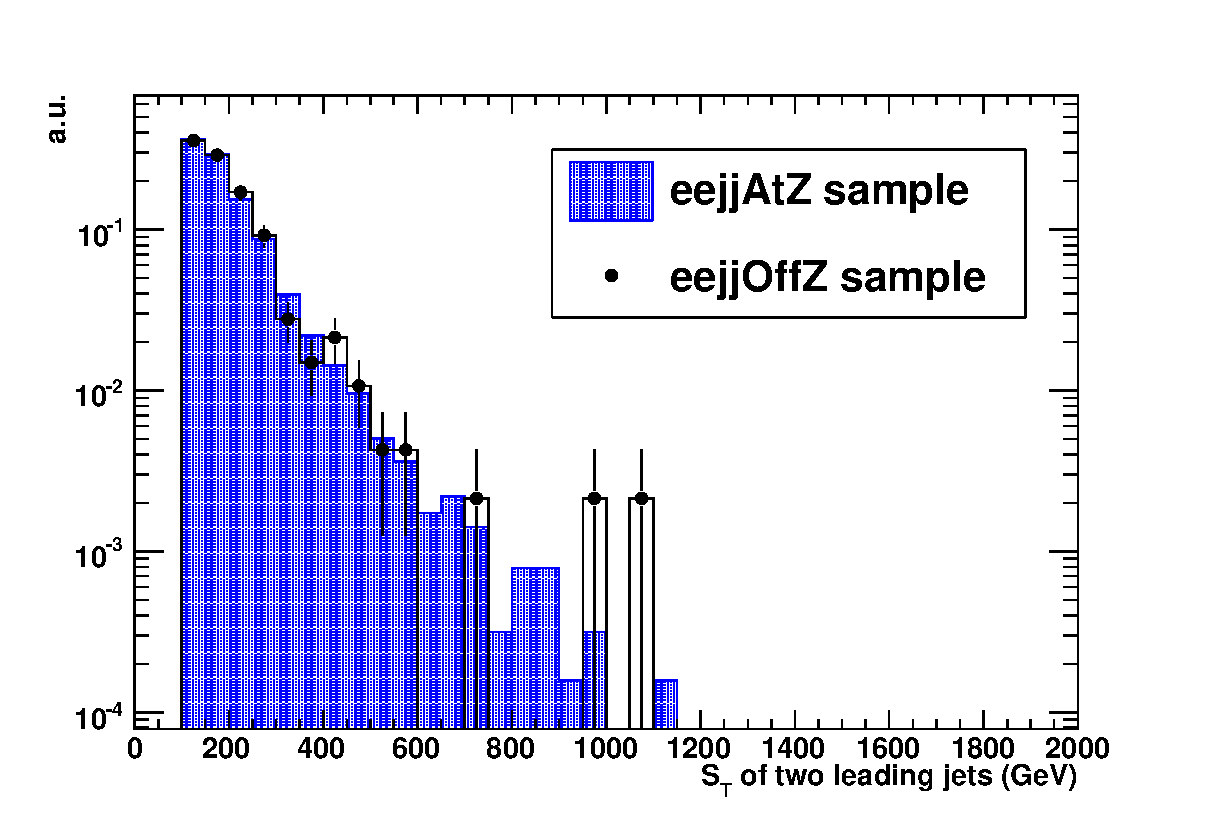
\includegraphics{plots/ZjetStudies/ST2jets_OffZvsAtZ_STcut300.eps}} &
    b.
    \resizebox{8cm}{!}{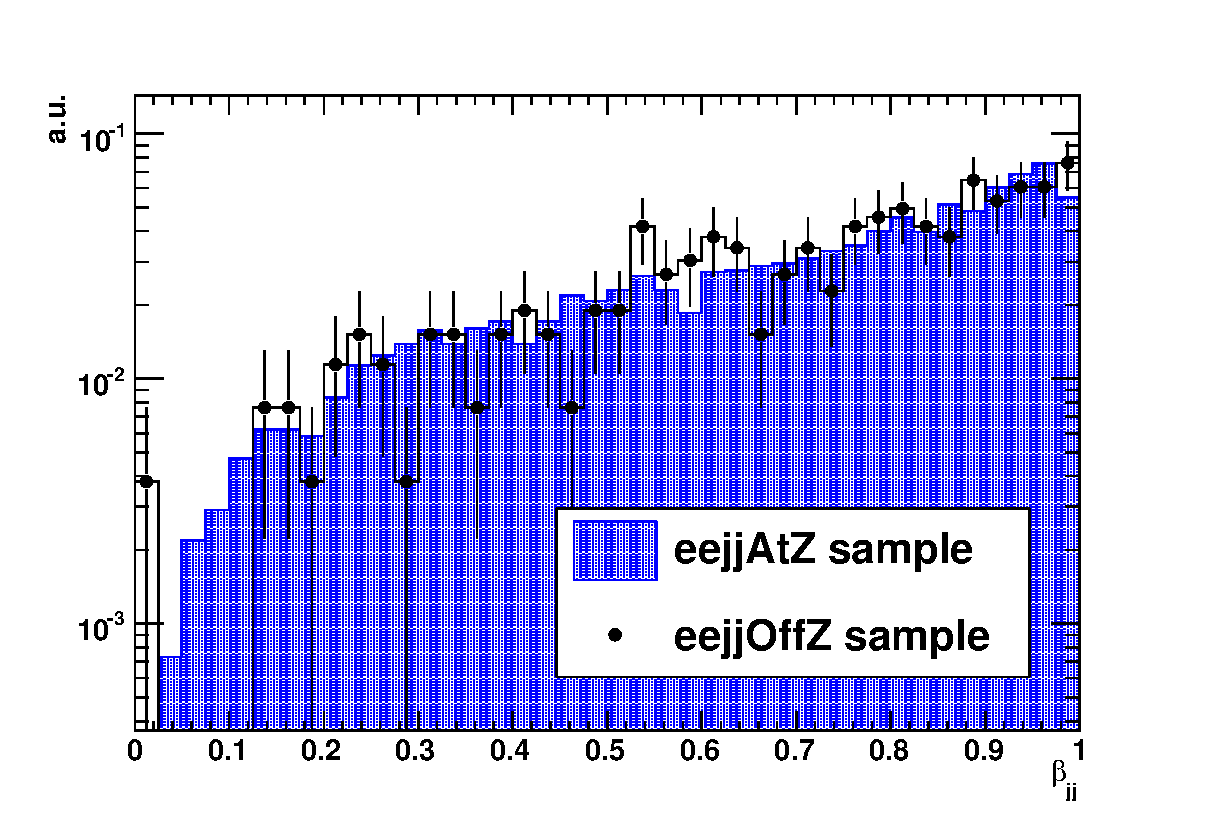
\includegraphics{plots/ZjetStudies/betajj_OffZvsAtZ_STcut300.eps}} \\
  \end{tabular}
  \caption{\small \sl Distributions of (a) $S_{T}^{jet}$ (b) $\beta_{jj}$ 
    for the eejjOffZ sample ($M_{ee} > 100\mbox{ GeV}$) 
    and the eejjAtZ control sample ($80\mbox{ GeV} < M_{ee} < 100\mbox{ GeV}$), 
    using a large FastSim sample of $Z/\gamma$+jet events. 
    The baseline selection of electrons and jets is applied in the first plot; 
    in addition, an $S_{T}$ cut of 300 GeV is applied in the second plot.}
  \label{fig:BjjSTJetseejjAtZvsOffZ}
  \end{center}
\end{figure}
%
%
%\begin{figure}[htb]
%  \begin{center}
%  \begin{tabular}{cc}
%    a.
%    \resizebox{8cm}{!}{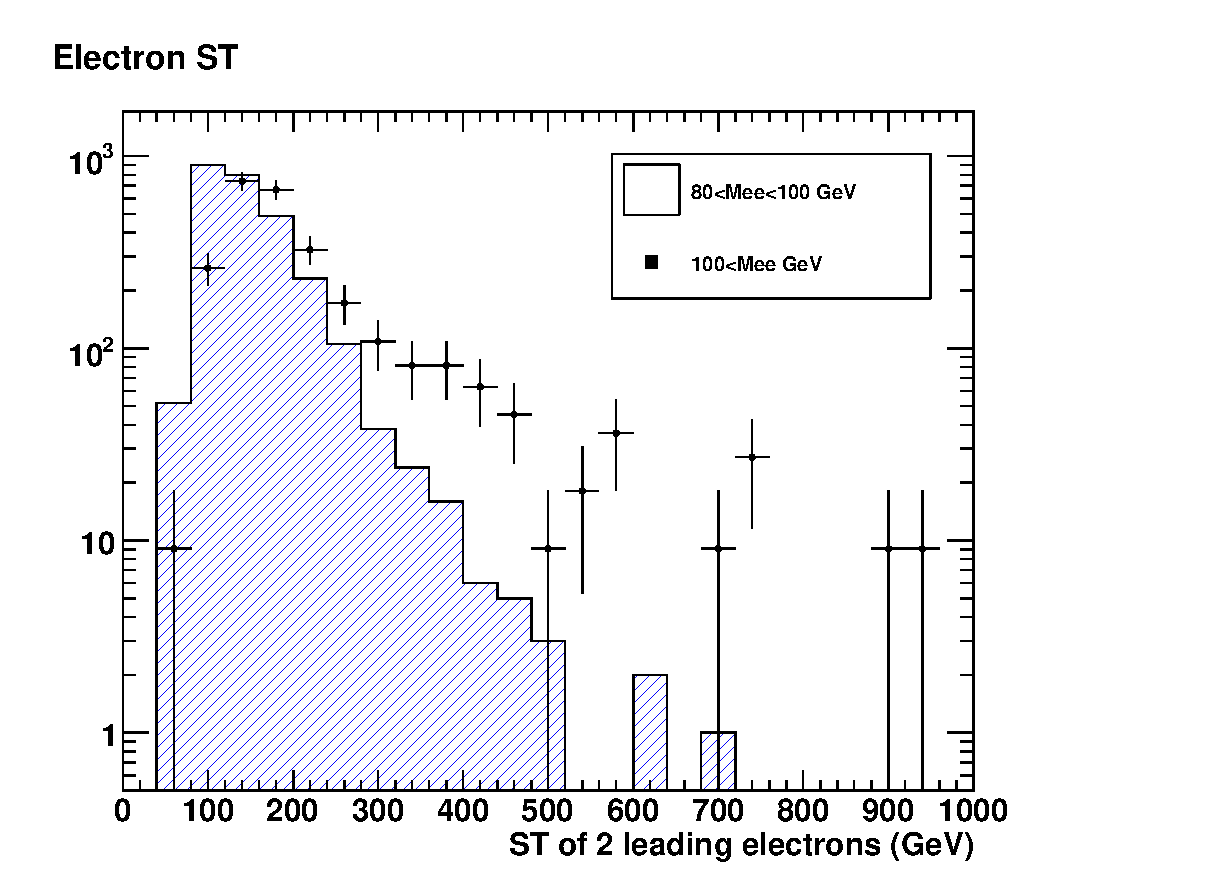
\includegraphics{plots/ZjetStudies/ST_Elecs_inside.eps}} &
%    b.
%    \resizebox{8cm}{!}{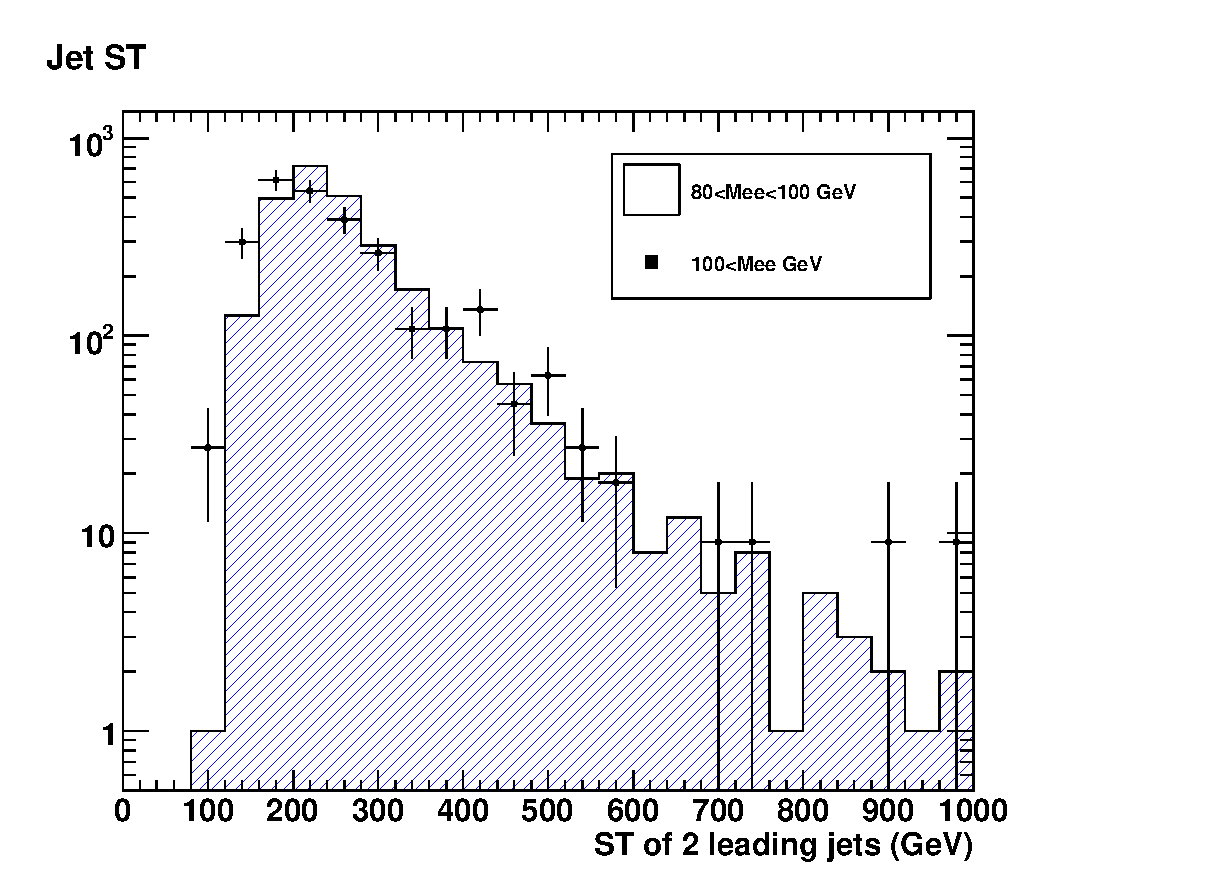
\includegraphics{plots/ZjetStudies/ST_Jets_inside.eps}} \\
%  \end{tabular}
%  \caption{\small \sl Distributions of (a) $S_{T}^{ele}$ (b) $S_{T}^{jet}$ 
%    for the signal eejj sample ($M_{ee} > 100\mbox{ GeV}$) 
%    and the eejjAtZ control sample ($80\mbox{ GeV} < M_{ee} < 100\mbox{ GeV}$), 
%    using a large FastSim sample of $Z/\gamma$+jet events.}
%  \label{fig:BjjSTJetseejjAtZvsOffZ}
%  \end{center}
%\end{figure}
%
%
%%%%%%%%%%%%%%%%%%% RATIO PLOT  %%%%%%%%%%%%%%%%%%%%

\begin{figure}[htb]
  \begin{center}
  \begin{tabular}{cc}
    a.
    \resizebox{8cm}{!}{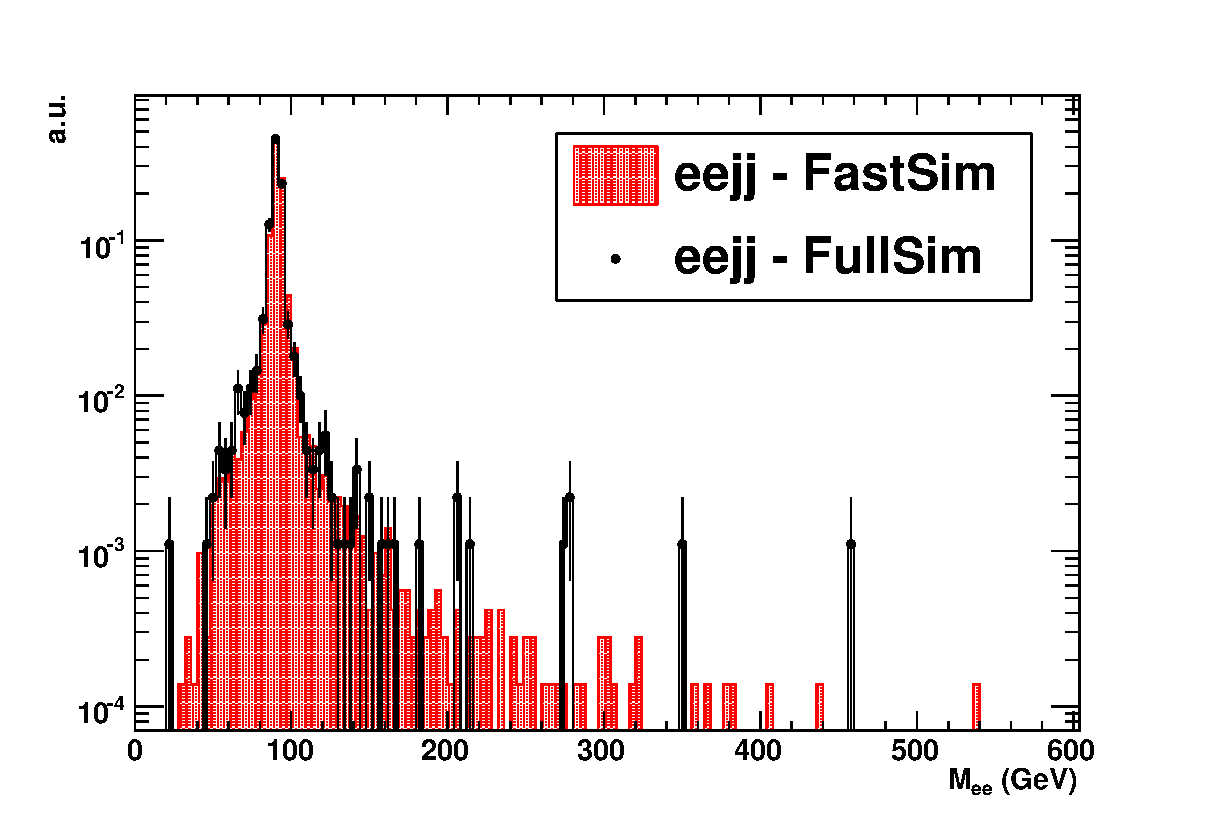
\includegraphics{plots/ZjetStudies/Mee_FastSimvsFullSim_pTjet50_pTele30_etaJet3.eps}} & 
    b.
    \resizebox{8cm}{!}{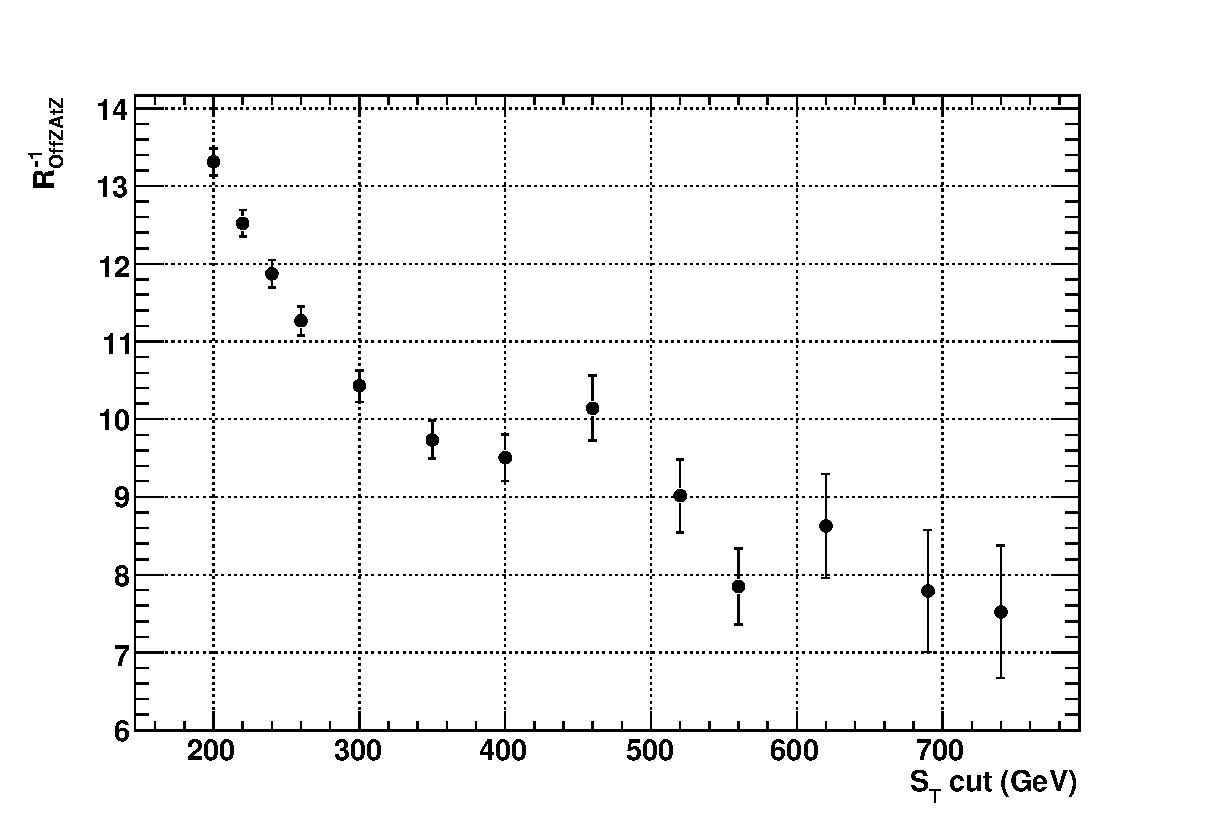
\includegraphics{plots/ZjetStudies/ratioInverseOffZAtZ.eps}} \\ 
  \end{tabular}
  \caption{\small \sl (a) the $M_{ee}$ distribution for FastSim and FullSim MC $Z/\gamma$+jet 
    events after the baseline selection 
    on electrons and jets described in Section~\ref{sec:eventSelection}, 
    (b) the value of the inverse of $R_{OffZ/AtZ}$ 
    as a function of different $S_{T}$ cuts, obtained from the FastSim MC sample of $Z/\gamma$+jet events.}
  \label{fig:ZJetRatioAndMeeFastVSFull}
  \end{center}
\end{figure}

%%%%%%%%%%%%%%%%%%%%%%%%%%%%%%%%%%%%%%%%%%%%%%
%
%
%%%%%%% CLOSURE TEST TABLE  %%%%%%%%%%%%%%%%

\begin{table}[htbp]
\begin{center}
\begin{tabular}{||c||c|c|c||c||}
\hline\hline
$S_{T}$ cut  &  $N_{eejjAtZ}$  &   $R_{OffZ/AtZ}^{-1}$  &     $N_{eejj}^{Z}$  &   $N_{eejjOffZ}$  \\ 
 (GeV)       &     (``data'')  &        (MC - FastSim)  &   (``data'' \& MC)  &   (MC - FullSim)  \\ 
\hline\hline
   200  &     278  $\pm$   16.67  &   13.31  $\pm$    0.17  &   20.88  $\pm$    1.28  &   22.21  $\pm$    2.84  \\ 
   220  &     252  $\pm$   15.87  &   12.52  $\pm$    0.17  &   20.12  $\pm$    1.30  &   22.21  $\pm$    2.84  \\ 
   240  &     221  $\pm$   14.87  &   11.87  $\pm$    0.18  &   18.62  $\pm$    1.28  &   21.11  $\pm$    2.77  \\ 
   260  &     187  $\pm$   13.67  &   11.26  $\pm$    0.18  &   16.60  $\pm$    1.24  &   19.29  $\pm$    2.65  \\ 
   300  &     129  $\pm$   11.36  &   10.43  $\pm$    0.21  &   12.37  $\pm$    1.12  &   13.47  $\pm$    2.21  \\ 
   350  &      87  $\pm$    9.33  &    9.73  $\pm$    0.24  &    8.94  $\pm$    0.98  &    8.37  $\pm$    1.75  \\ 
   400  &      52  $\pm$    7.21  &    9.51  $\pm$    0.30  &    5.47  $\pm$    0.78  &    5.46  $\pm$    1.41  \\ 
%   440  &      36  $\pm$    6.00  &   10.15  $\pm$    0.38  &    3.55  $\pm$    0.61  &    3.64  $\pm$    1.15  \\ 
   460  &      30  $\pm$    5.48  &   10.14  $\pm$    0.42  &    2.96  $\pm$    0.55  &    2.55  $\pm$    0.96  \\ 
%   480  &      27  $\pm$    5.20  &   10.32  $\pm$    0.46  &    2.62  $\pm$    0.52  &    2.18  $\pm$    0.89  \\ 
   520  &      21  $\pm$    4.58  &    9.01  $\pm$    0.47  &    2.33  $\pm$    0.52  &    1.09  $\pm$    0.63  \\ 
   560  &      16  $\pm$    4.00  &    7.85  $\pm$    0.49  &    2.04  $\pm$    0.53  &    0.73  $\pm$    0.52  \\ 
   620  &      11  $\pm$    3.32  &    8.63  $\pm$    0.67  &    1.28  $\pm$    0.40  &    0.73  $\pm$    0.52  \\ 
   690  &       6  $\pm$    2.45  &    7.79  $\pm$    0.78  &    0.77  $\pm$    0.32  &    0.73  $\pm$    0.52  \\ 
   740  &       4  $\pm$    2.00  &    7.52  $\pm$    0.85  &    0.53  $\pm$    0.27  &    0.36  $\pm$    0.36  \\ 
\hline\hline
\end{tabular}
\end{center}
\caption{\small \sl The results of the data driven method for $Z/\gamma$+jet background 
estimate assuming 100 pb$^{-1}$ of data. $N_{eejjAtZ}$ is the number of events in the eejjAtZ control sample 
(here obtained from the FullSim MC sample of $Z/\gamma$+jet events), the statistical uncertainty 
on this number is $\sqrt{N_{eejj}^{Z}}$; $R_{OffZ/AtZ}^{-1}$ is the inverse of the 
ratio between number of ``OffZ'' divided by ``AtZ'' $Z/\gamma$+jet events obtained from the FastSim MC sample; 
$N_{eejj}^{Z}$ is the estimate of $Z/\gamma$+jet events in the eejj sample obtained from the data driven method by 
Equation~\ref{formula:NeejjZ}; $N_{eejjOffZ}$ is the number of 
events passing the full eejj selection directly obtained from the FullSim MC sample of $Z/\gamma$+jet events. 
The quantities described above are given for different values of the $S_T$ cut.}
\label{tab:ZjetClosureTest}
\end{table}


%\begin{figure}
%  \begin{center}
%  \begin{tabular}{cc}
%  \resizebox{10cm}{!}{
\includegraphics{plots/UMD.eps}} \\ 
%  \end{tabular}
%  \caption{\small \sl Distribution of the $p_{T}$ at generator level of the electron pair ($p_{T}$ of the boson) 
%    for $Z/\gamma$+jet events in the signal eejj sample 
%    (cut 1,2,3,4)
%    and the control sample (cut 1,2,4 + $80\mbox{ GeV} < M_{ee} < 100\mbox{ GeV}$), for $Z/\gamma$+jet events.}
%  \label{fig:pTeePair}
%  \end{center}
%\end{figure}

%http://cmssw.cvs.cern.ch/cgi-bin/cmssw.cgi/CMSSW/Configuration/CSA07Production/data/CSA07_zjet_ptjgt20_Rmatch0.7_excl.cfg?revision=1.2&view=markup

%alpgen
%zjet_0ptz100gen
%z2j_0ptz100
%njets 2
%ebeam 7000
%ih2 1  - for proton/proton collisions
%ickkw 1 - CKKW prescription for the running of alphas's in the extra gluon emission processes	
%iqopt 1 - renormalization scale
%ptjmin 20
%etajmax 5
%drjmin 0.7
%izdecmode 4

%Fit method (histogram, unbinned, function, combination...)

\clearpage

\subsection{QCD Multi-jet Background} \label{sec:QCDBackground}

%% The MC statistics of the QCD multi-jet sample is not sufficient to perform a reasonable estimate of the contamination 
%% of QCD events in the eejj sample.
%% %, although it seems to confirm the expectation that it is small compared with 
%% %the dominant $t\bar{t}$ and $Z/\gamma$+jet backgrounds (see Table~\ref{tab:EventSelSummary}). 
%% In addition, large uncertainties are expected on the cross section of QCD production at LHC start-up.
%% For this reason different techniques (possibly data-driven) are preferred to estimate the QCD background.

The MC samples of the QCD multi-jet background are generated in four bins of $H_T$, as shown in Table~\ref{tab:NumEvents}.
For each bin, the selection efficiencies and the number of events in 100 pb$^{-1}$ passing the eejj selection 
(optimized for LQ mass of 400 GeV) are reported in Tables 
\ref{tab:effic-QCD-100-250},
\ref{tab:effic-QCD-250-500},
\ref{tab:effic-QCD-500-1000} and
\ref{tab:effic-QCD-1000-inf}. 
The number of surviving QCD multi-jet events goes to zero rapidly as the selection is applied. 
Only in the sample with $H_T\in[500,1000]$~GeV one single event survives the full selection, corresponding
to $0.37\pm 0.37$ events in 100 pb$^{-1}$.
In order to estimate this background with an increased statistical precision, a factorized 
method based on Monte Carlo is used.

A QCD multi-jet sample with two fake electrons and two jets (ffjj sample)
that pass all the kinematic selection criteria (see Section~\ref{sec:eventSelection}) is selected and 
rescaled to estimate the QCD multi-jet contamination in the eejj sample as

%
\begin{equation} \label{QCDRescaling}
N_{eejj}^{QCD} = N_{ffjj}^{QCD} \times {P(e|f)}^2 \quad , 
\end{equation}
%

where ``f'' is a reconstructed electron with loose ID requirements (all objects in the initial electron collection 
before applying HEEP ID and Isolation), 
``e'' is a reconstructed electron which pass all the HEEP ID and Isolation criteria (see Table~\ref{tab:HEEPselection} 
of Section~\ref{sec:IdAndIso}), 
$N_{eejj}^{QCD}$ ($N_{ffjj}^{QCD}$) is the number of QCD multi-jet events in the eejj (ffjj) sample (control sample), 
and $P(e|f)$ is the probability of a fake electron (f) to pass the HEEP ID and Isolation requirements (e).

%% The probability $P(e|f)$ is obtained from a ffjj sample of QCD events (QCD ($H_T\in[500,1000]$~GeV) is used 
%% since it's the largest contribution in the control sample), by dividing the total number of ``e'' candidates in the sample 
%% by the total number of ``f'' candidates. 
Table~\ref{tab:ffjjSelection} summarizes 
the absolute number of events passing the ffjj selection, the number 
of selected events rescaled to 100 pb$^{-1}$ of data, the cross section at LO 
and the equivalent integrated luminosity of each $H_T$ 
bin of the QCD multi-jet sample. 
The total number of ffjj events in 100 pb$^{-1}$ of data is $N_{ffjj}^{QCD}=6130 \pm 47$.
An $S_{T}$ cut of 460 GeV (which is the optimized cut value for LQ mass of 250 GeV) is used in 
the ffjj selection.
Since $S_{T} \approx H_T$, this kinematically excludes any 
QCD multi-jet contribution from the sample generated in the lowest $H_T$ bin of $[100,250]$~GeV. 
Therefore, only the three remaining $H_T$ bins are used.

\begin{table}[htbp]
\begin{center}
\begin{tabular}{|l|c|c|c|c|}
\hline\hline
 $H_T$ bin (GeV)   & $N_{evt}^{sel}$ & $N_{evt}^{sel}$ for 100pb$^{-1}$ & $\sigma_{LO}$ (pb) & Equivalent           \\
                         &                 &                                  &                    & Luminosity (pb$^{-1}$) \\
\hline\hline
$[250,500]$              &  4              & 43.3    $\pm$ 21.6               & $400 \times 10^3$  &  9.25                \\
$[500,1000]$             &  12431          & 4571.6  $\pm$ 40.9               & $14 \times 10^3$   &  272                 \\
$>1000$                  &  26786          & 1515.1  $\pm$ 9.1                & $370$              &  1.77$\times 10^3$   \\
\hline\hline
\end{tabular}
\end{center}
\caption{Number of selected events in the ffjj sample for different $H_T$ bins of the QCD multi-jet sample.}
\label{tab:ffjjSelection}
\end{table}


The probability $P(e|f)$ is estimated from the rate of ``f'' to ``e'' in a ffjj sample obtained
from the QCD multi-jet samples by applying the selection cuts described in 
Section~\ref{sec:eventSelection} with the $S_T$ cut set to 460~GeV.
%(QCD ($H_T\in[500,1000]$~GeV) is used since it's the largest contribution in the control sample).
In the barrel region ($|\eta|<1.5$), the probability $P(e|f)$ is almost flat in $\eta$ and $\approx 2.5 \cdot 10^{-3}$,  
while in the endcap region it is increasing with $\eta$ and has an average value of $\approx 1.4 \cdot 10^{-2}$.
%up to $\approx 3 \cdot 10^{-2}$ for $|\eta|=2.5$. 
The overall average value in barrel and endcaps is $P(e|f) = 5.3 \cdot 10^{-3}$.
A closure test performed without isolation cuts suggests 
that this method might underestimate the 
%value of $P(e|f)$ by about 20\%.
QCD multi-jet background by approximately 40\%.
%A possible reason for this discrepancy is that, by applying Equation~\ref{QCDRescaling}
%with a constant value of $P(e|f)$, we are not taking into account $\eta$ and $p_T$ dependencies.
%Keeping this into account we can state that $P(e|f)$ is within the range $[5.3, 6.5] \cdot 10^{-3}$.

%An uncertainty of 200\% on the value of $P(e|f)$ is estimated 
%from closure tests performed with relaxed ID and Isolation cuts.

With the cut $S_T>460$~GeV, the number of QCD multi-jet events in the eejj sample is estimated as 
$0.17<N_{eejj}^{QCD}<0.26$ events by rescaling the ffjj sample 
with Equation~\ref{QCDRescaling} and 
%using the above range for $P(e|f)$. 
taking into account the underestimation suggested by the closure test.
%this value is in agreement with the estimate of $0.37 \pm 0.37$ events 
%(see Table~\ref{tab:EventSelSummary}) obtained by directly applying the full eejj 
%selection on the QCD MC sample. 
Therefore, QCD multi-jet background is expected to be small compared to 
the $t\bar{t}$ and $Z/\gamma$+jet backgrounds for the same $S_T$ cut, 
as shown in Table~\ref{tab:EventSelSummary}. 
It has been verified that this statement remains true even when a harder $S_T$ cut is applied.
For example, the number of QCD multi-jet background events estimated with the described technique
becomes $0.026<N_{eejj}^{QCD}<0.039$ with $S_T>740$~GeV.

The contamination of QCD multi-jet background in the e$\mu$jj sample 
is expected to be even smaller than eejj sample, since the probability for jets to fake muons 
is smaller than for electrons. %FIXME REFERENCE FOR MUON FAKE RATE%

The method described above currently relies on MC. 
It is foreseen in future upgrades of the analysis to use a full data driven technique where 
both ffjj control sample and $P(e|f)$ are extracted from data. 

%\end{document}
